\chapter{Lenguaje: ArchiMate}
\section{Introducción}
Para el desarrollo de proyectos de ingeniería de software se requiere una serie de componentes, pasos y estructura bien definida que debe seguirse para llevar a buen término la finalización del mismo. Una de estas partes fundamentales en la ingeniería de software es el lenguaje de modelado, el cual es un lenguaje artificial que puede ser utilizado para expresar la información o el conocimiento o sistemas en una estructura que se define por un conjunto coherente de normas. Las reglas se utilizan para interpretar el significado de los componentes de la estructura. Estos lenguajes de modelado pueden ser de dos tipos en específico, el primero es el gráfico, el cual utiliza una técnica de diagrama con símbolos con nombre que representan conceptos y líneas que conectan los símbolos y representan relaciones y varias otras notaciones gráficas para representar restricciones. y el lenguaje textual que puede usar palabras clave estandarizadas acompañadas de parámetros o términos y frases en lenguaje natural para hacer expresiones interpretables por computadora. Entre estos lenguajes de modelado se encuentra uno muy útil el cual es ArchiMate, el cual consiste en un amplio, abierto e independiente lenguaje de modelado con el fin de apoyar la descripción, análisis y visualización de la arquitectura deentro del proyecto de fóma veráz y efectiva. ArchiMate es un estándar técnico de The Open Group y se basa en los conceptos del estándar IEEE 1471 . Cuenta con el respaldo de varios proveedores de herramientas y empresas consultoras. ArchiMate también es una marca registrada de The Open Group. Open Group tiene un programa de certificación para usuarios de ArchiMate, herramientas de software y cursos. ArchiMate se distingue de otros lenguajes como el Lenguaje de modelado unificado (UML) y el Modelado y notación de procesos de negocio (BPMN) por su alcance de modelado empresarial.

\begin{figure}[h!]
	\centering
	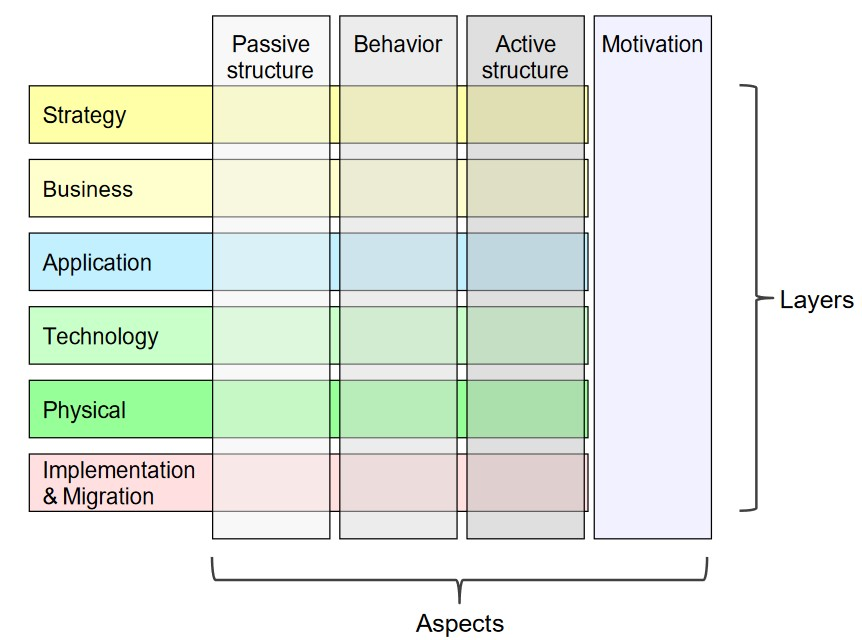
\includegraphics[width=0.7\linewidth]{imgs/coreFramwork}
	\caption{Marco completo de ArchiMate}
\end{figure}

\section{Conceptos y su notación}
El lenguaje ArchiMate separa los conceptos del lenguaje (es decir, los constituyentes del metamodelo) de su notación. Diferentes grupos de interesados pueden requerir diferentes notaciones para comprender un modelo o una visión de la arquitectura.  A este respecto, los ArchiMatelanguages de lenguajes como el UML o el BPMN, que sólo tienen una notación normalizada. El mecanismo de punto de vista explicado en el Capítulo 14 proporciona los medios para definir tales visualizaciones orientadas a las partes interesadas. Aunque la notación de los conceptos de ArchiMate puede (y debería) ser específica de las partes interesadas, la norma proporciona una notación gráfica común, que puede ser utilizada por los arquitectos y otros que desarrollan modelos ArchiMate. Esta notación está dirigida a un público acostumbrado a las técnicas de modelización técnica existentes, como ERD, UML o BPMN, y por lo tanto se asemeja a ellas. En el resto de este documento, a menos que se indique lo contrario, los símbolos utilizados para representar los conceptos del lenguaje representan la notación estándar de ArchiMate.  Esta notación estándar para la mayoría de los elementos consiste en un cuadro con un icono en la esquina superior derecha. En varios casos, este icono por sí mismo puede también utilizarse como notación alternativa. Esta iconografía estándar debe preferirse siempre que sea posible para que cualquier persona que conozca el lenguaje ArchiMate pueda leer los diagramas producidos en el lenguaje.

\subsection{Meta}

La principal jerarquía de elementos de comportamiento y estructura del lenguaje ArchiMate se presenta en la tabla 3.1. Define estos elementos de forma genérica e independiente de la capa. Nótese que la mayoría de estos elementos (las cajas blancas) son elementos abstractos del metamodelo; es decir, no están instanciados en los modelos sino que sólo sirven para estructurar el metamodelo.  La notación presentada es, por lo tanto, la forma genérica en que se representan las especializaciones de estos elementos (es decir, los elementos de las diferentes capas de la arquitectura). Además de describir  los elementos concretos (los recuadros grises), que pueden utilizarse para modelar la Arquitectura de la Empresa a nivel estratégico.

\newpage
\subsubsection{Elementos de la Estructura}
	\begin{table}[h!]
	\begin{tabular}{| m{7em} | m{7cm} | m{3cm} |}
		\hline
		Concepto & Descripción & Representación \\
		
		\hline
		Motivación
		& 
		Un elemento de motivación representa el contexto o la motivación detrás de la  arquitectura de la empresa
		& 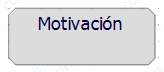
\includegraphics[width=0.8\linewidth, height=0.05\textheight]{imgs/conceptos/meta/Motivacion}
		\\
		
		\hline
		Estructura 
		& 
		Elementos de estructura son equivalentes sinónimos, se subdividen  en estructuras activas ,                              estructuras activas internas,  estructuras activas externas y estructuras pasivas
		& 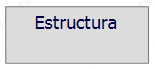
\includegraphics[width=0.8\linewidth, height=0.05\textheight]{imgs/conceptos/meta/Estructura}
		\\
		
		\hline
		Estructura activa  
		& 
		Estructuras que pueden tener un comportamiento
		& 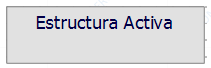
\includegraphics[width=0.8\linewidth, height=0.05\textheight]{imgs/conceptos/meta/EstructuraActiva}
		\\  
		
		\hline
		Estructura activa externa  
		& 
		Llamado interfase representa un punto de acceso donde uno o mas servicios son prestados al ambiente  
		&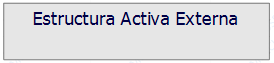
\includegraphics[width=0.8\linewidth, height=0.05\textheight]{imgs/conceptos/meta/EstructuraActivaExterna}
		\\
		
		\hline
		Estructura activa interna
		& 
		Es un elemento que representa una entidad que es capaz de mostrar comportamiento
		& 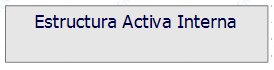
\includegraphics[width=0.8\linewidth, height=0.05\textheight]{imgs/conceptos/meta/EstructuraActivaInterna.PNG}
		\\
		
		\hline
		Estructura pasiva
		& 
		Es un elemento que representa una entidad sobre la cual se realiza un comportamiento
		& 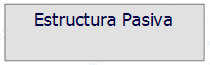
\includegraphics[width=0.8\linewidth, height=0.05\textheight]{imgs/conceptos/meta/EstructuraPasiva.PNG}
		\\
		
		\hline
		Interfase
		& 
		Representa un punto de acceso donde uno o mas servicios son puestos en el ambiente.
		& 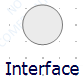
\includegraphics[width=0.8\linewidth, height=0.05\textheight]{imgs/conceptos/meta/Interface.PNG}
		\\
		
		\hline
		
		Comportamiento
		& 
		Es un elemento que equivale a un verbo se  subdivide en evento ,comportamiento interno, proceso , función, interacción, comportamiento externo y servicio.
		& 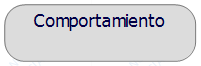
\includegraphics[width=0.8\linewidth, height=0.05\textheight]{imgs/conceptos/meta/Comportamiento.PNG}
		\\
		
		\hline
		Evento
		&
		Representa un cambio de estado 
		& 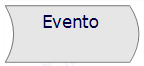
\includegraphics[width=0.8\linewidth, height=0.05\textheight]{imgs/conceptos/meta/Evento.PNG}
		\\
		
		\hline
		Elemento de comportamiento interno 
		& 
		Representa una o mas unidades de actividades que pueden ser realizadas por uno o mas elementos de estructura activa
		& 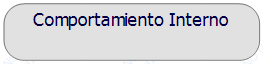
\includegraphics[width=0.8\linewidth, height=0.05\textheight]{imgs/conceptos/meta/ComportamientoInterno.PNG}
		\\	\hline
	\end{tabular}
	%\caption{}
	\label{tab:concepts}
\end{table}

\newpage
\begin{table}[h!]
\begin{center}
	\begin{tabular}{| m{6em} | m{7cm} | m{3cm} |}
		\hline
		Concepto & Descripción & Representación \\ 
		
		\hline
		Servicio
		&
		Un servicio es un comportamiento del sistema proveedor  visible  externamente 
		&
		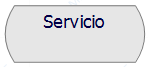
\includegraphics[width=0.8\linewidth, height=0.05\textheight]{imgs/conceptos/meta/Servicio.PNG}
		\\
		
		\hline
		Función
		& 
		Representa una colección de comportamientos, basado en una colección de criterios específicos, tales como fuente requerida, competencias o localización   
		& 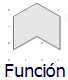
\includegraphics[width=0.8\linewidth, height=0.05\textheight]{imgs/conceptos/meta/Funcion.PNG}
		\\
		
		\hline
		Proceso
		& 
		Representa una secuencia de comportamientos que consiguen un resultado especifico
		& 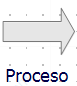
\includegraphics[width=0.8\linewidth, height=0.05\textheight]{imgs/conceptos/meta/Proceso.PNG}
		\\
		
		\hline
		Interacción  
		& 
		Representa una unidad de comportamientos que deben ser realizados por dos o mas elementos de estructura activa interna , ya sea a través de una asignación directa o agregados en una colaboración 
		& 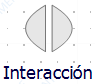
\includegraphics[width=0.8\linewidth, height=0.05\textheight]{imgs/conceptos/meta/Interaccion.PNG}
		\\
		
		\hline
		Colaboración  
		& 
		Representa un acuerdo entre dos o mas elementos estructuras activas internas, trabajan juntos para realizar algún comportamiento colectivo   
		& 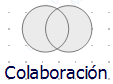
\includegraphics[width=0.8\linewidth, height=0.05\textheight]{imgs/conceptos/meta/Colaboracion.PNG}
		\\
		
		\hline
		Elemento de comportamiento externo
		& 
		Representa un comportamiento explicito que es visible en el exterior  
		& 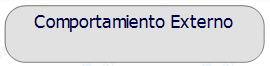
\includegraphics[width=0.8\linewidth, height=0.05\textheight]{imgs/conceptos/meta/ComportamientoExterno.PNG}
		\\
		
		\hline
		
		Elementos compuestos 
		&
		Son elementos que se basan en aspectos de otras capas del lenguaje   
		&
		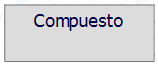
\includegraphics[width=0.8\linewidth, height=0.05\textheight]{imgs/conceptos/meta/Compuesto.PNG}
		\\
		
		\hline
	\end{tabular}
	\caption{Conceptos capa meta}
	\label{tab:concepts}
\end{center}
\end{table}

\newpage
\subsection{Motivación}

Los elementos de motivación se utilizan para modelar las motivaciones, o razones, que guían el diseño o el cambio de una Arquitectura Empresarial. Es esencial entender los factores, a menudo denominados impulsores, que influyen en otros elementos de motivación.  Pueden originarse tanto dentro como fuera de la empresa.  Los impulsores internos, también llamados preocupaciones, están asociados con las partes interesadas, que pueden ser algún ser humano individual o algún grupo de seres humanos, como un equipo de proyecto, una empresa o la sociedad. Ejemplos de esos impulsores internos son la satisfacción del cliente, el cumplimiento de la legislación o la rentabilidad. Es común que las empresas realicen una evaluación de esos factores impulsores; por ejemplo, utilizando un análisis FODA, a fin de responder de la mejor manera posible.

\begin{center}
	\begin{tabular}{ | m{6em} | m{4cm}| m{2cm} | } 
		\hline
		Motivación& Un elemento que proporciona el contexto o la razón detrás de la arquitectura de una empresa & 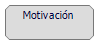
\includegraphics[width=0.8\linewidth, height=0.05\textheight]{imgs/Elementos/Motivacion.PNG}
		\\ 
		\hline
	\end{tabular}
\end{center}

\newpage
\subsubsection{Elementos de la Estructura}
\begin{table}[h!]
	\begin{center}
		\begin{tabular}{| m{6em} | m{7cm}| m{3cm} |}
			\hline
			Concepto & Descripción & Representación \\ 
			\hline
			
			Implicado 
			& 
			El papel de un individuo, equipo u organización (o clases de los mismos) que representa sus intereses en el resultado de la arquitectura 
			& 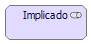
\includegraphics[width=0.8\linewidth, height=0.05\textheight]{imgs/Elementos/Implicado.PNG}
			\\
			\hline
			Manejador 
			& 
			Una condición externa o interna que motiva a una organización para definir sus galones e implementar los cambios necesarios para lograrlos. 
			& 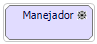
\includegraphics[width=0.8\linewidth, height=0.05\textheight]{imgs/Elementos/Manejador.PNG}
			\\
			\hline
			Valoración 
			& 
			El resultado de un análisis de la situación de la empresa con respecto a algún conductor. 
			& 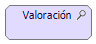
\includegraphics[width=0.8\linewidth, height=0.05\textheight]{imgs/Elementos/Valoracion.PNG}
			\\
			\hline
			Objetivo 
			& 
			Una declaración de intención, dirección o estado final deseado de alto nivel para una organización y sus partes interesadas. 
			& 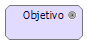
\includegraphics[width=0.8\linewidth, height=0.05\textheight]{imgs/Elementos/Objetivo.PNG}
			\\
			\hline
			Resultado 
			& 
			Un resultado final que se ha logrado
			& 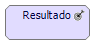
\includegraphics[width=0.8\linewidth, height=0.05\textheight]{imgs/Elementos/Resultado.PNG}
			\\
			\hline
			Principio 
			& 
			Una declaración cualitativa de intenciones que debe ser satisfecha por la arquitectura
			& 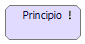
\includegraphics[width=0.8\linewidth, height=0.05\textheight]{imgs/Elementos/Principio.PNG}
			\\
			\hline
			Requerimiento 
			& 
			Una declaración de necesidad que debe ser satisfecha por la arquitectura
			& 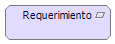
\includegraphics[width=0.8\linewidth, height=0.05\textheight]{imgs/Elementos/Requerimiento.PNG}
			\\
			\hline
			Restricción 
			& 
			Un factor que previene oUn factor que previene u obstruye laUn factor que previene u obstruye la realizaciónUn factor que previene u obstruye la realización de metas
			& 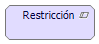
\includegraphics[width=0.8\linewidth, height=0.05\textheight]{imgs/Elementos/Restriccion.PNG}
			\\
			\hline
			Significado 
			& 
			Los conocimientos o la experiencia presentes en, o la interpretación dada a, un elemento
			& 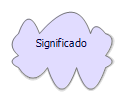
\includegraphics[width=0.8\linewidth, height=0.05\textheight]{imgs/Elementos/Significado.PNG}
			\\
			\hline
			Valor 
			& 
			El valor relativo, la utilidad o la importancia de un elemento básico o un resultado
			& 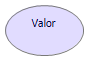
\includegraphics[width=0.8\linewidth, height=0.05\textheight]{imgs/Elementos/Valor.PNG}
			\\
			
			\hline
		\end{tabular}
		\caption{Conceptos Capa Motivacional}
		\label{tab:concepts}
	\end{center}
\end{table}

\subsection{Punto de Vista Estratégico}
Para describir los aspectos de la estrategia de nuestra empresa, se explicaran los siguientes puntos de vista presentado diferentes perspectivas de la aplicación del modelo a la dirección de nuestra empresa:
\subsubsection{Punto de vista de estrategia}
\begin{table}[th!]
	\begin{center}
		\begin{tabular}{| c | p{6cm} |} %r c|}
			\hline
			\multicolumn{2}{ |c| }{Punto de vista de la estrategia}
			
			\\ \hline
			
			Stakeholders
			& 
			CxOs(Chief eXperience Officer), gerentes del negocio y arquitectos empresariales y de negocio. 
			
			\\ \hline
			Ocupaciones 
			& 
			Desarrollador de estrategias.
			
			\\ \hline
			
			Propósito 
			& 
			Desarrollo y toma de decisiones.
			
			\\ \hline
			
			Alcance 
			& 
			Estrategia. 
			
			\\ \hline
			
			Elementos relacionados 
			& 
			Cursos de acción, capacidad, flujo del valor, recurso, Outcomes.     		
			
			\\ \hline
		\end{tabular}
		\caption{Descripción del punto de vista de estrategia}
	\end{center}
\end{table}

\subsubsection{Punto de vista del mapeado de las capacidades}
\par Permite mostrar un punto de vista general de las capacidades de la empresa; típicamente el mapeado nos muestra 2 o 3 niveles de las capacidades de una empresa, por ejemplo se puede crear un mapeado de calor que nos muestre áreas de inversión, además en algunos casos nos permite especificar las salidas con sus determinadas capacidades.
\begin{table}[th!]
	\begin{center}
		\begin{tabular}{| c | p{8cm} |} %r c|}
			\hline
			\multicolumn{2}{ |c| }{mapeado de las capacidades}
			
			\\ \hline
			
			Stakeholders
			& 
			Gerentes del negocio y arquitectos empresariales y de negocio. 
			
			\\ \hline
			Ocupaciones 
			& 
			Arquitecto de estrategias, tácticas y motivación.
			
			\\ \hline
			
			Propósito 
			& 
			Desarrollo y toma de decisiones.
			
			\\ \hline
			
			Alcance 
			& 
			Estrategia. 
			
			\\ \hline
			
			Elementos relacionados 
			& 
			capacidad, recurso, Outcomes.     		
			
			\\ \hline
		\end{tabular}
		\caption{Descripción del punto de vista del mapeado de las capacidades}
	\end{center}
\end{table}

\subsubsection{Punto de vista del flujo del valor}
\par Permite mostrar un punto de vista general del flujo del valor; Identifica las capacidades que soportan las etapas en el flujo del valor, valor creado y stakeholders involucrados.
\begin{table}[th!]
	\begin{center}
		\begin{tabular}{| c | p{8cm} |} %r c|}
			\hline
			\multicolumn{2}{ |c| }{Flujo del valor}
			
			\\ \hline
			
			Stakeholders
			& 
			Gerentes del negocio y arquitectos empresariales y de negocio. 
			
			\\ \hline
			Ocupaciones 
			& 
			Arquitecto de estrategias, tácticas y motivación.
			
			\\ \hline
			
			Propósito 
			& 
			Desarrollo y toma de decisiones.
			
			\\ \hline
			
			Alcance 
			& 
			Estrategia. 
			
			\\ \hline
			
			Elementos relacionados 
			& 
			capacidad, flujo del valor, Outcomes, stakeholders.     		
			
			\\ \hline
		\end{tabular}
		\caption{Descripción del punto de vista del flujo del valor}
	\end{center}
\end{table}

\subsubsection{Punto de vista realización de resultados}
\par Este punto de vista es usado para mostrar el nivel más alto de la arquitectura, muestra los negocios orientados a los resultados producidos por las capacidades y los elementos adyacentes al núcleo de la empresa.
\begin{table}[th!]
	\begin{center}
		\begin{tabular}{| c | p{8cm} |} %r c|}
			\hline
			\multicolumn{2}{ |c| }{Realización de resultados}
			
			\\ \hline
			
			Stakeholders
			& 
			Gerentes del negocio y arquitectos empresariales y de negocio. 
			
			\\ \hline
			Ocupaciones 
			& 
			Negocios orientados a resultados.
			
			\\ \hline
			
			Propósito 
			& 
			Desarrollo y toma de decisiones.
			
			\\ \hline
			
			Alcance 
			& 
			Estrategia. 
			
			\\ \hline
			
			Elementos relacionados 
			& 
			capacidad, flujo del valor, recursos, Outcomes, valor, aceptación, elementos del núcleo.     		
			
			\\ \hline
		\end{tabular}
		\caption{Descripción punto de vista de realización de resultados}
	\end{center}
\end{table}

\subsubsection{Punto de vista mapeado de recursos}
\par Permite crear y estructurar una visión general de los recursos de la empresa; típicamente el mapeado nos muestra 2 o 3 niveles de las capacidades de una empresa, por ejemplo se puede crear un mapeado de calor que nos muestre áreas de inversión, además en algunos casos nos permite especificar las relaciones entre los recursos y las capacidades asignadas.
\begin{table}[th!]
	\begin{center}
		\begin{tabular}{| c | p{8cm} |} %r c|}
			\hline
			\multicolumn{2}{ |c| }{mapeado de recursos}
			
			\\ \hline
			
			Stakeholders
			& 
			Gerentes del negocio y arquitectos empresariales y de negocio. 
			
			\\ \hline
			Ocupaciones 
			& 
			Arquitecto de estrategias, tácticas y motivación.
			
			\\ \hline
			
			Propósito 
			& 
			Desarrollo y toma de decisiones.
			
			\\ \hline
			
			Alcance 
			& 
			Estrategia. 
			
			\\ \hline
			
			Elementos relacionados 
			& 
			capacidad,recursos, paquetes de trabajo.     		
			
			\\ \hline
		\end{tabular}
		\caption{Descripción punto de vista mapeado de recursos}
	\end{center}
\end{table}

\subsection{Negocio}

La Capa de Negocios se utiliza típicamente (en conjunto con los elementos de estrategia) para modelar la arquitectura de negocios de una empresa, definida por el marco del TOGAF como una descripción de la estructura e interacción entre la estrategia de negocios, la organización, las funciones, los procesos de negocios y las necesidades de información.

\subsubsection{Elementos de la Estructura}
\begin{table}[H]
	\centering
	\begin{tabular}{| m{3cm} | m{7cm} | m{3.8cm} |}
		\hline
		\textbf{Concepto}           & \textbf{Definición} & \textbf{Notación} \\ \hline
		
		Actor de Negocios        & Una entidad organizacional que es capaz de ejecutar un comportamiento.                                                                                                              &\vspace{1.52mm}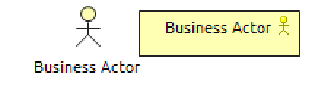
\includegraphics[width=40mm, height=10mm]{imgs/conceptos/negocio/Business_actor.pdf}    \\ \hline
		
		Rol de Negocios          & La responsabilidad de tener un comportamiento especifico, ante el cual un actor puede ser asignado.                                                                                 &\vspace{1.52mm}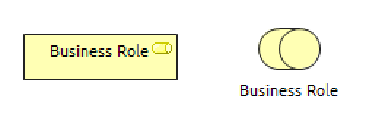
\includegraphics[width=40mm, height=10mm ]{imgs/conceptos/negocio/Business_role.pdf}         \\ \hline
		
		Colaboración de Negocios & Un agregado de dos o más roles de negocios que trabajan juntos para tener un comportamiento colectivo.                                                                             
		&\vspace{1.52mm} 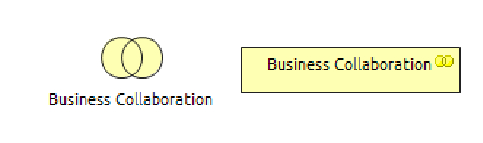
\includegraphics[width=40mm,height=10mm]{imgs/conceptos/negocio/Business_colaboration.pdf}             \\ \hline
		
		Interfaz de Negocios     & Un punto de acceso donde un servicio comercial está disponible para su entorno.                                                                                                     
		&\vspace{1.52mm}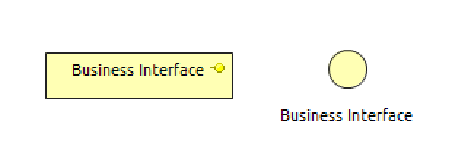
\includegraphics[width=40mm,height=10mm]{imgs/conceptos/negocio/Business_Interface.pdf}  \\ \hline
		
		Ubicación                & Un punto conceptual en el espacio.                                                                                     
		&\vspace{1.52mm}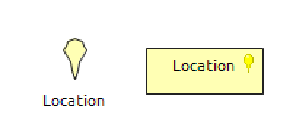
\includegraphics[width=40mm, height=10mm]{imgs/conceptos/negocio/Location.pdf}           \\ \hline
		
		Objeto de Negocios       & Un elemento pasivo que tiene relevancia desde una perspectiva de negocios.                                                                                                         
		&\vspace{1.52mm}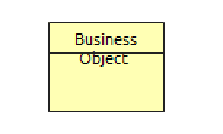
\includegraphics[width=40mm, height=10mm]{imgs/conceptos/negocio/Business_Object.pdf}   \\ \hline
		
		Proceso de Negocios      & Un elemento de comportamiento que agrupa el comportamiento basado en un orden de actividades. Es destinado a producir un  conjunto definido de productos o servicios comerciales.
		&\vspace{1.52mm} 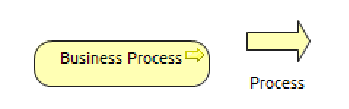
\includegraphics[width=40mm, height=10mm]{imgs/conceptos/negocio/Business_proces.pdf}            \\ \hline
		
		Función de Negocios      & Un elemento de comportamiento que agrupa el comportamiento basado en un conjunto de criterios elegidos (típicamente recursos comerciales requeridos y / o competencias).        &\vspace{1.52mm}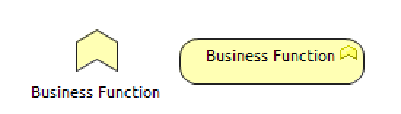
\includegraphics[width=40mm, height=10mm]{imgs/conceptos/negocio/Business_function.pdf}            \\ \hline
		
		Interacción de Negocios  & Un elemento de comportamiento que describe la conducta de una colaboración empresarial.                                                                                             
		&\vspace{1.52mm} 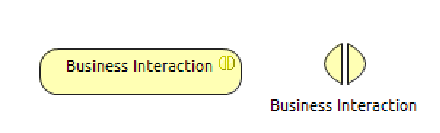
\includegraphics[width=40mm,height=10mm]{imgs/conceptos/negocio/Business_interaction.pdf}            \\ \hline
		
		Evento de Negocios       & Algo que sucede (internamente o externamente) e influye en el  comportamiento.                                                                                                       
		&\vspace{1.52mm} 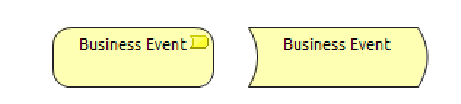
\includegraphics[width=40mm, height=10mm]{imgs/conceptos/negocio/Business_event.pdf}  \\ \hline
		
	\end{tabular}
\end{table}

\newpage
\begin{table}[H]
	\centering
	\begin{tabular}{| m{3cm} | m{7cm} | m{3.8cm} |}
		\hline
		\textbf{Concepto}           & \textbf{Definición} & \textbf{Notación} \\ \hline
		
		Servicio de Negocios     & Un servicio que satisface una necesidad comercial de un cliente (interno o externo al organización).        &\vspace{2mm}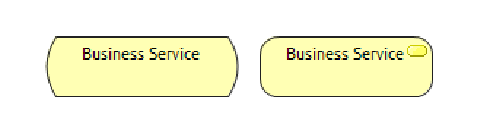
\includegraphics[width=40mm, height=8mm]{imgs/conceptos/negocio/Business_service.pdf}  \\ \hline
		
		Representación           & Una forma perceptible de la información llevado por un objeto de negocios.                                                                                                           &\vspace{1.52mm}  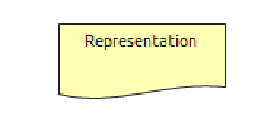
\includegraphics[width=40mm, height=10mm]{imgs/conceptos/negocio/Representation.pdf}            \\ \hline
		Significado              & El conocimiento o experiencia presente en un objeto de negocios o su representación, dado un contexto particular.                                                                   &\vspace{1.52mm}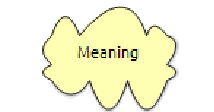
\includegraphics[width=40mm, height=8mm]{imgs/conceptos/negocio/Meaning.pdf}           \\ \hline
		
		Valor                    & El valor relativo, la utilidad o la importanciade un servicio o producto comercial.                                                                                                  
		&\vspace{1.52mm}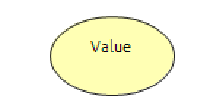
\includegraphics[width=40mm, height=10mm]{imgs/conceptos/negocio/Value.pdf}        \\ \hline
		
		Producto                 & Una colección coherente de servicios, acompañado de un contrato / conjunto de acuerdos, que se ofrece en su conjunto para (internos o externos) clientes.                           &\vspace{1.52mm}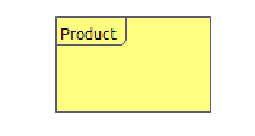
\includegraphics[width=40mm, height=10mm]{imgs/conceptos/negocio/Product.pdf}         \\ \hline
		
		Contrato                 & Una especificación formal o informal de acuerdo que especifica los derechos y obligaciones asociadas con un producto.                                                                 &\vspace{1.52mm}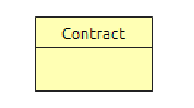
\includegraphics[width=40mm, height=10mm]{imgs/conceptos/negocio/Contract.pdf}       \\ \hline
		
	\end{tabular}
\end{table}

\subsection{Punto de Vista de la Aplicación}
El punto de vista de Aplicación describe el comportamiento interno de una aplicación; por ejemplo, cuando realiza uno o más servicios de aplicación.

\subsubsection{Punto de Vista de comportamiento}
Este punto de vista es útil para diseñar el comportamiento principal de las aplicaciones o para identificar la superposición funcional entre diferentes aplicaciones. Se preocupa por la estructura, relaciones y dependencias entre aplicaciones, consistencia e integridad, reducción de complejidad de la aplicación
\begin{figure}[th!]
	\centering
	\fcolorbox{black}{white}{
		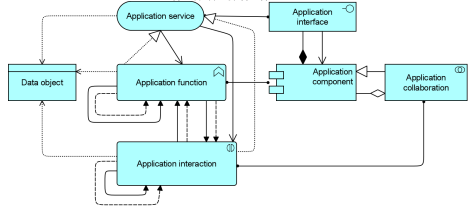
\includegraphics[width=0.9\linewidth]{imgs/puntos_vista/aplicacion/vistacomportamiento}}
	\caption{vista de comportamiento de aplicación}
	\label{fig:vistaaplicacion}
\end{figure}

\subsubsection{Punto de Vista de cooperacion}
El punto de vista de la cooperación de aplicaciones describe las relaciones entre los componentes de las aplicaciones en términos de los flujos de información entre ellos, o en términos de los servicios que ofrecen y utilizan. Este punto de vista se utiliza normalmente para crear una descripción general del panorama de aplicaciones de una organización. Este punto de vista también se utiliza para expresar la cooperación interna o la orquestación de servicios que en conjunto apoyan la ejecución de un proceso empresarial.

\begin{figure}[th!]
	\centering
	\fcolorbox{black}{white}{
		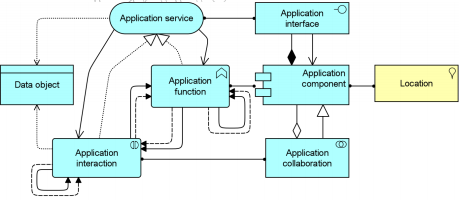
\includegraphics[width=0.9\linewidth]{imgs/puntos_vista/aplicacion/vistacooperacion}}
	\caption{vista de cooperacion de aplicación}
	\label{fig:vistaaplicacion}
\end{figure}

\subsubsection{Punto de Vista de estructura}
El punto de vista Estructura de la aplicación muestra la estructura de una o más aplicaciones o componentes. 
Este punto de vista es útil para diseñar o comprender la estructura principal de aplicaciones o componentes y los datos asociados; p. ej., para desglosar la estructura del sistema en construcción o para identificar componentes de aplicaciones heredados que son adecuados para la migración / integración
\begin{figure}[th!]
	\centering
	\fcolorbox{black}{white}{
		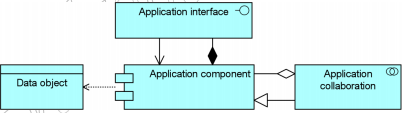
\includegraphics[width=0.9\linewidth]{imgs/puntos_vista/aplicacion/vistaestructura}}
	\caption{vista de estructura de aplicación}
	\label{fig:vistaaplicacion}
\end{figure}	

\subsubsection{Punto de Vista de uso}
El punto de vista Uso de aplicaciones describe cómo se utilizan las aplicaciones para dar soporte a uno o más procesos de negocio y cómo las utilizan otras aplicaciones. 
Se puede utilizar para diseñar una aplicación identificando los servicios que necesitan los procesos de negocio y otras aplicaciones, o para diseñar procesos de negocio al describir los servicios que están disponibles. 

\subsection{Punto de Vista de la Tecnología}
El punto de vista de infraestructura general, trata acerca del hardware y la infraestructura de comunicación que soporta la capa de aplicación. Esta capa ofrece servicios de infraestructura requeridos para desplegar las aplicaciones realizadas en los ordenadores y los sistemas de
hardware y software.



\subsubsection{Punto de vista de uso de infraestructura}

El punto de vista de uso de infraestructura muestra como las aplicaciones son soportadas por la infraestructura de software y hardware: los servicios de infraestructura son entregados por los dispositivos, los sistemas de software y redes son entregados a las aplicaciones. Este
punto de vista juega un rol importante en el análisis del rendimiento y la escalabilidad y puede ser usado para determinar requerimientos de rendimiento y calidad en la infraestructura basado en las demandas de las aplicaciones que la usan.
\newpage

\begin{figure}[h]
	\centering
	\fcolorbox{black}{white}{
		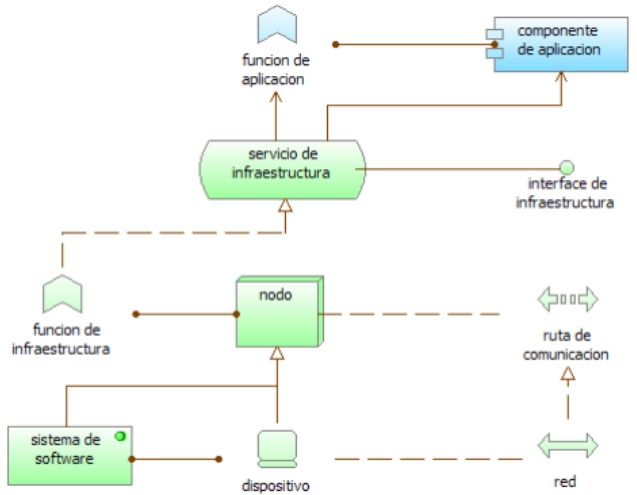
\includegraphics[width=0.5\linewidth]{imgs/puntos_vista/tecnologia/MMDUDI.jpg}}
	\caption{Metamodelo de uso de infraestructura}
\end{figure}

\subsubsection{Modelo de uso de infraestructura}

En este punto de vista se identifican los servicios de infraestructura principales que corresponden al servicio de notificaciones, generar reportes, establecer tiempos de acceso a la
aplicación, y gestionar los usuarios. Cada uno de los servicios de infraestructura entrega configuración y la funcionalidad requerida hacia los componentes de aplicación.


\begin{figure}[h]
	\centering
	\fcolorbox{black}{white}{
		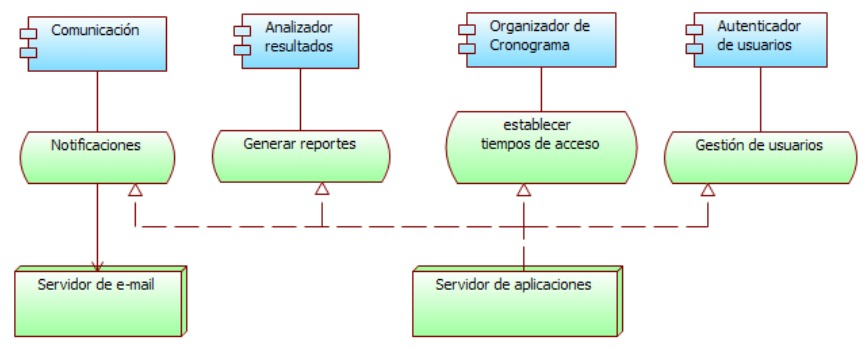
\includegraphics[width=0.5\linewidth]{imgs/puntos_vista/tecnologia/MDUDI.jpg}}
	\caption{Modelo de uso de infraestructura}
\end{figure}



\subsubsection{ Punto de vista de Implementación y despliegue}
El punto de vista de implementación y despliegue muestra como uno o más aplicaciones son realizadas sobre la infraestructura. Esto implica el mapeo de aplicaciones (lógicas) y componentes en artefactos (físicos). Esta vista juega un papel importante en el análisis del rendimiento y la escalabilidad debido a la relación entre la infraestructura y el mundo lógico de las aplicaciones.


\begin{figure}[h]
	\centering
	\fcolorbox{black}{white}{
		\includegraphics[width=0.5\linewidth]{imgs/puntos_vista/tecnologia/MMDIYD.jpg}}
	\caption{Metamodelo de implementación y despliegue}
\end{figure}

\subsubsection{Modelo de implementación y despliegue}

En este punto de vista, se muestra como todos los componentes son realizados por el nodo de servidor de aplicaciones, el componente de comunicación va a ser realizado por el nodo servidor de aplicaciones y tiene una relación de asociación con el nodo servidor de e-mail que
proveerá las configuraciones de software específico para el envío de notificaciones, resultados e información sobre el proceso.

\begin{figure}[h]
	\centering
	\fcolorbox{black}{white}{
		\includegraphics[width=0.5\linewidth]{imgs/puntos_vista/tecnologia/MDIYD.jpg}}
	\caption{Modelo de implementación y despliegue}
\end{figure}



\begin{table}[h]
	\begin{center}
		\begin{tabular}{ | m{7em} | m{8cm}|  } 
			\hline
			Interesados & Arquitectos de infraestructura, gerentes operativos 
			\\
			\hline
			Preocupaciones & Estabilidad, seguridad, dependencias, costos de la infraestructura
			\\
			\hline
			Propósito & Diseñar
			\\
			\hline
			Alcance & Una capa / aspecto múltiple
			\\
			\hline
		\end{tabular}
		\caption{Punto de Vista Tecnología}
		\label{tab:concepts}
	\end{center}
\end{table}

\textbf{Elementos que participan: }
\begin{itemize}
	\item Ubicación
	\item Nodo
	\item Colaboración tecnológica
	\item Dispositivo
	\item Software del sistema
	\item Interfaz tecnológica
	\item Red de comunicacion
	\item Camino
	\item Proceso tecnológico / función / interacción
	\item Servicio de tecnología
	\item Evento tecnológico
	\item Artefacto
\end{itemize}

\subsection{Físico}

Estos se basan en la Capa de Tecnología. No se definen elementos de comportamiento físico separados.  Más bien, los elementos de comportamiento de la Capa de Tecnología (función de la tecnología, proceso, interacción, servicio y evento) se usan para modelar el comportamiento de todos los nodos, incluyendo el equipo físico. Dado que el equipo muy a menudo estará controlado por computadora o tendrá una estrecha relación con la tecnología de la información (piense también en los sensores, Internet de las cosas), su comportamiento puede describirse de manera integral utilizando los conceptos de comportamiento de la tecnología existente.

\newpage
\subsubsection{Elementos de la Estructura}

\begin{longtable}{|c| c| c|}
	\hline
	Concepto & Descripción & Representación \\ \hline
	Facilidad
	&
	\begin{tabular}{p{6cm}p{3cm}}
		Representa un recurso físico que tiene la capacidad de
		facilitar (por ejemplo, albergar o ubicar) el uso de equipos. Por lo general, se utiliza para modelar fábricas, edificios o construcciones al aire libre
	\end{tabular} 
	& \includegraphics[width=0.1\linewidth, height=0.05\textheight]{imgs/conceptos/fisico/facilidad}
	\\
	\hline 
	Equipo
	& 
	\begin{tabular}{p{6cm}p{3cm}}
		El equipo comprende todos los elementos de procesamiento activos que llevan a cabo procesos físicos en los que se utilizan o transforman materiales.
	\end{tabular} 
	& \includegraphics[width=0.1\linewidth, height=0.05\textheight]{imgs/conceptos/fisico/equipo}
	\\
	\hline
	Red de distribución
	&
	\begin{tabular}{p{6cm}p{3cm}} 
		Representa la distribución física o la infraestructura de transporte. Encarna la realización física de las rutas lógicas entre nodos. Una red de distribución conecta dos o más nodos. Una red de distribución puede realizar uno o más caminos.
	\end{tabular} 
	& \includegraphics[width=0.1\linewidth, height=0.05\textheight]{imgs/conceptos/fisico/redDistribucion}
	\\
	\hline
	Material
	&
	\begin{tabular}{p{6cm}p{3cm}}  
		El material representa materia física tangible, con atributos como tamaño y peso. Suele utilizarse para modelar materias primas y productos físicos, y también fuentes de energía como el combustible.
	\end{tabular}
	& \includegraphics[width=0.1\linewidth, height=0.05\textheight]{imgs/conceptos/fisico/material}
	\\
	\hline
\end{longtable}

\section{Relaciones}

el lenguaje ArchiMate define un conjunto básico de relaciones genéricas, cada una de las cuales puede conectar un conjunto predefinido de conceptos de origen y destino (en la mayoría de los casos elementos, pero en unos pocos casos también otras relaciones).  Muchas de estas relaciones están "sobrecargadas"; es decir, su significado exacto difiere según los conceptos de origen y destino que conectan, y se clasifican de la siguiente manera:
\begin{itemize}
	\item Relaciones estructurales, que modelan la construcción o composición estática de conceptos del mismo o diferentes tipos.
	\item Relaciones de dependencia, que modelan cómo se utilizan los elementos para apoyar otros elementos.
	\item Las relaciones dinámicas, que se utilizan para modelar las dependencias de comportamiento entre los elementos.
	\item Otras relaciones, que no entran en ninguna de las categorías anteriores.
\end{itemize}

\subsection{Relaciones Estructurales}

Las relaciones estructurales representan la coherencia "estática" dentro de una arquitectura.  El concepto de composición (el lado "de" de la relación) es siempre un elemento; el concepto de composición (el lado "de" de la relación) puede en algunos casos ser también otra relación.

\begin{table}[h!]
	\subsubsection{Elementos}
	\begin{center}
		\begin{tabular}{| l | l | r |}
			\hline
			Concepto & Descripción & Representación \\ \hline
			
			Agregación 
			&
			\begin{tabular}[l]{@{}l@{}}
				Indica que un elemento consiste en \\
				uno u otros conceptos más.
			\end{tabular}
			& \includegraphics[width=0.4\linewidth]{imgs/relaciones/agregacion}
			\\\hline
			
			Composición
			& 
			\begin{tabular}[l]{@{}l@{}}
				Indica que un elemento consiste en \\
				uno u otros conceptos más.
			\end{tabular}
			& \includegraphics[width=0.4\linewidth]{imgs/relaciones/composicion}
			\\\hline
			
			Asignación
			& 
			\begin{tabular}[l]{@{}l@{}}
				Expresa la asignación de \\
				responsabilidad, la ejecución \\
				de la conducta, o la ejecución.
			\end{tabular}
			& \includegraphics[width=0.4\linewidth]{imgs/relaciones/asignacion}
			\\\hline
			
			Realización
			& 
			\begin{tabular}[l]{@{}l@{}}
				Indica que una entidad desempeña \\
				un papel fundamental en la creación,\\
				el logro, el sustento o el \\
				funcionamiento de una entidad más \\
				abstracta.
			\end{tabular}
			& \includegraphics[width=0.4\linewidth]{imgs/relaciones/realizacion}
			\\\hline
			
		\end{tabular}
		\caption{Relaciones estructurales}
		\label{tab:estructurales}
	\end{center}
\end{table}

\subsection{Relaciones de Dependencia}

Las relaciones de dependencia describen la forma en que los elementos apoyan o son utilizados por otros elementos.  Se distinguen tres tipos de relaciones de dependencia:
\begin{itemize}
	\item La relación de servicio representa una dependencia de control, denotada por una línea sólida.
	\item La relación de acceso representa una dependencia de datos, denotada por una línea discontinua.
	\item La relación de influencia es el tipo de dependencia más débil, utilizada para modelar cómo los elementos de motivación son influenciados por otros elementos.
\end{itemize}
Obsérvese que, aunque la notación de estas relaciones se asemeja a la notación de la relación de dependencia en UML, estas relaciones tienen significados distintos en la notación ArchiMate y (normalmente) apuntan en la dirección opuesta.

\begin{table}[h!]
	\subsubsection{Elementos}
	\begin{center}
		\begin{tabular}{| c | l | l |}
			\hline
			Concepto & Descripción & Representación \\ \hline
			
			Sirve 
			&
			\begin{tabular}{m{12em}}
				Modela que un elemento proporciona
				su funcionalidad a otro elemento.
			\end{tabular}
			& \includegraphics[width=0.4\linewidth]{imgs/relaciones/sirve}
			\\\hline
			
			Influencia
			& 
			\begin{tabular}{m{12em}}
				Modelos en los que un elemento afecta la aplicación o el logro
				de algún elemento de motivación.
			\end{tabular}
			& \includegraphics[width=0.4\linewidth]{imgs/relaciones/influencia}
			\\\hline
			
			Acceso
			& 
			\begin{tabular}{m{12em}}
				Modela la capacidad de los elementos
				de comportamiento y estructura activa
				para observar o actuar sobre los
				elementos de estructura pasiva.
			\end{tabular}
			& \includegraphics[width=0.4\linewidth]{imgs/relaciones/acceso}
			\\\hline
			
			Acceso Bidireccional
			& 
			\begin{tabular}{m{12em}}
				Modela la capacidad de los elementos
				de comportamiento y estructura activa
				para observar o actuar sobre los
				elementos de estructura pasiva y viceversa.
			\end{tabular}
			& \includegraphics[width=0.4\linewidth]{imgs/relaciones/accesobi}
			\\\hline
			
		\end{tabular}
		\caption{Relaciones de dependencia}
		\label{tab:dependencia}
	\end{center}
\end{table}

\subsection{Relaciones Dinámicas}

Las relaciones dinámicas describen las dependencias temporales entre los elementos de la arquitectura. Se distinguen dos tipos de relaciones dinámicas: de activación y de flujo.

\begin{table}[h]
	\subsubsection{Elementos}
	\begin{center}
		\begin{tabular}{| l | l | r |}
			\hline
			Concepto & Descripción & Representación \\ \hline
			
			Flujo 
			&
			\begin{tabular}[l]{@{}l@{}}
				Transferencia de un elemento a otro.
			\end{tabular}
			& \includegraphics[width=0.4\linewidth]{imgs/relaciones/flujo}
			\\\hline
			
			Disparo
			& 
			\begin{tabular}[l]{@{}l@{}}
				Describe una relación temporal o \\
				causal entre los elementos.
			\end{tabular}
			& \includegraphics[width=0.4\linewidth]{imgs/relaciones/disparo}
			\\\hline
			
		\end{tabular}
		\caption{Relaciones dinámicas}
		\label{tab:dinamicas}
	\end{center}
\end{table}


\subsection{Otras Relaciones}

\begin{table}[h]
	\subsubsection{Elementos}
	\begin{center}
		\begin{tabular}{| l | l | c |}
			\hline
			Concepto & Descripción & Representación \\ \hline
			
			Asociación 
			&
			\begin{tabular}[l]{@{}l@{}}
				Modela una relación no especificada, \\
				o una que no está representado por \\
				otro ArchiMate relación.
			\end{tabular}
			& \includegraphics[width=0.4\linewidth]{imgs/relaciones/asociacion}
			\\\hline
			
			Especialización
			& 
			\begin{tabular}[l]{@{}l@{}}
				Indica que un elemento es un tipo \\
				particular de otro elemento.
			\end{tabular}
			& \includegraphics[width=0.4\linewidth]{imgs/relaciones/especializacion}
			\\\hline
			
			Unión
			& 
			\begin{tabular}[l]{@{}l@{}}
				Se usa para conectar relaciones \\
				del mismo tipo.
			\end{tabular}
			& \includegraphics[width=0.2\linewidth]{imgs/relaciones/union}
			\\\hline
			
		\end{tabular}
		\caption{Otras relaciones}
		\label{tab:otras}
	\end{center}
\end{table}

\section{Puntos de Vista}

\newpage
\subsection{Motivación}

Los elementos de motivación se utilizan para modelar las motivaciones, o razones, que guían el diseño o el cambio de una Arquitectura Empresarial. Es esencial entender los factores, a menudo denominados impulsores, que influyen en otros elementos de motivación.  Pueden originarse tanto dentro como fuera de la empresa.  Los impulsores internos, también llamados preocupaciones, están asociados con las partes interesadas, que pueden ser algún ser humano individual o algún grupo de seres humanos, como un equipo de proyecto, una empresa o la sociedad. Ejemplos de esos impulsores internos son la satisfacción del cliente, el cumplimiento de la legislación o la rentabilidad. Es común que las empresas realicen una evaluación de esos factores impulsores; por ejemplo, utilizando un análisis FODA, a fin de responder de la mejor manera posible.

\begin{center}
	\begin{tabular}{ | m{6em} | m{4cm}| m{2cm} | } 
		\hline
		Motivación& Un elemento que proporciona el contexto o la razón detrás de la arquitectura de una empresa & \includegraphics[width=0.8\linewidth, height=0.05\textheight]{imgs/Elementos/Motivacion.PNG}
		\\ 
		\hline
	\end{tabular}
\end{center}

\newpage
\subsubsection{Elementos de la Estructura}
\begin{table}[h!]
	\begin{center}
		\begin{tabular}{| m{6em} | m{7cm}| m{3cm} |}
			\hline
			Concepto & Descripción & Representación \\ 
			\hline
			
			Implicado 
			& 
			El papel de un individuo, equipo u organización (o clases de los mismos) que representa sus intereses en el resultado de la arquitectura 
			& \includegraphics[width=0.8\linewidth, height=0.05\textheight]{imgs/Elementos/Implicado.PNG}
			\\
			\hline
			Manejador 
			& 
			Una condición externa o interna que motiva a una organización para definir sus galones e implementar los cambios necesarios para lograrlos. 
			& \includegraphics[width=0.8\linewidth, height=0.05\textheight]{imgs/Elementos/Manejador.PNG}
			\\
			\hline
			Valoración 
			& 
			El resultado de un análisis de la situación de la empresa con respecto a algún conductor. 
			& \includegraphics[width=0.8\linewidth, height=0.05\textheight]{imgs/Elementos/Valoracion.PNG}
			\\
			\hline
			Objetivo 
			& 
			Una declaración de intención, dirección o estado final deseado de alto nivel para una organización y sus partes interesadas. 
			& \includegraphics[width=0.8\linewidth, height=0.05\textheight]{imgs/Elementos/Objetivo.PNG}
			\\
			\hline
			Resultado 
			& 
			Un resultado final que se ha logrado
			& \includegraphics[width=0.8\linewidth, height=0.05\textheight]{imgs/Elementos/Resultado.PNG}
			\\
			\hline
			Principio 
			& 
			Una declaración cualitativa de intenciones que debe ser satisfecha por la arquitectura
			& \includegraphics[width=0.8\linewidth, height=0.05\textheight]{imgs/Elementos/Principio.PNG}
			\\
			\hline
			Requerimiento 
			& 
			Una declaración de necesidad que debe ser satisfecha por la arquitectura
			& \includegraphics[width=0.8\linewidth, height=0.05\textheight]{imgs/Elementos/Requerimiento.PNG}
			\\
			\hline
			Restricción 
			& 
			Un factor que previene oUn factor que previene u obstruye laUn factor que previene u obstruye la realizaciónUn factor que previene u obstruye la realización de metas
			& \includegraphics[width=0.8\linewidth, height=0.05\textheight]{imgs/Elementos/Restriccion.PNG}
			\\
			\hline
			Significado 
			& 
			Los conocimientos o la experiencia presentes en, o la interpretación dada a, un elemento
			& \includegraphics[width=0.8\linewidth, height=0.05\textheight]{imgs/Elementos/Significado.PNG}
			\\
			\hline
			Valor 
			& 
			El valor relativo, la utilidad o la importancia de un elemento básico o un resultado
			& \includegraphics[width=0.8\linewidth, height=0.05\textheight]{imgs/Elementos/Valor.PNG}
			\\
			
			\hline
		\end{tabular}
		\caption{Conceptos Capa Motivacional}
		\label{tab:concepts}
	\end{center}
\end{table}

\subsection{Punto de Vista Estratégico}
Para describir los aspectos de la estrategia de nuestra empresa, se explicaran los siguientes puntos de vista presentado diferentes perspectivas de la aplicación del modelo a la dirección de nuestra empresa:
\subsubsection{Punto de vista de estrategia}
\begin{table}[th!]
	\begin{center}
		\begin{tabular}{| c | p{6cm} |} %r c|}
			\hline
			\multicolumn{2}{ |c| }{Punto de vista de la estrategia}
			
			\\ \hline
			
			Stakeholders
			& 
			CxOs(Chief eXperience Officer), gerentes del negocio y arquitectos empresariales y de negocio. 
			
			\\ \hline
			Ocupaciones 
			& 
			Desarrollador de estrategias.
			
			\\ \hline
			
			Propósito 
			& 
			Desarrollo y toma de decisiones.
			
			\\ \hline
			
			Alcance 
			& 
			Estrategia. 
			
			\\ \hline
			
			Elementos relacionados 
			& 
			Cursos de acción, capacidad, flujo del valor, recurso, Outcomes.     		
			
			\\ \hline
		\end{tabular}
		\caption{Descripción del punto de vista de estrategia}
	\end{center}
\end{table}

\subsubsection{Punto de vista del mapeado de las capacidades}
\par Permite mostrar un punto de vista general de las capacidades de la empresa; típicamente el mapeado nos muestra 2 o 3 niveles de las capacidades de una empresa, por ejemplo se puede crear un mapeado de calor que nos muestre áreas de inversión, además en algunos casos nos permite especificar las salidas con sus determinadas capacidades.
\begin{table}[th!]
	\begin{center}
		\begin{tabular}{| c | p{8cm} |} %r c|}
			\hline
			\multicolumn{2}{ |c| }{mapeado de las capacidades}
			
			\\ \hline
			
			Stakeholders
			& 
			Gerentes del negocio y arquitectos empresariales y de negocio. 
			
			\\ \hline
			Ocupaciones 
			& 
			Arquitecto de estrategias, tácticas y motivación.
			
			\\ \hline
			
			Propósito 
			& 
			Desarrollo y toma de decisiones.
			
			\\ \hline
			
			Alcance 
			& 
			Estrategia. 
			
			\\ \hline
			
			Elementos relacionados 
			& 
			capacidad, recurso, Outcomes.     		
			
			\\ \hline
		\end{tabular}
		\caption{Descripción del punto de vista del mapeado de las capacidades}
	\end{center}
\end{table}

\subsubsection{Punto de vista del flujo del valor}
\par Permite mostrar un punto de vista general del flujo del valor; Identifica las capacidades que soportan las etapas en el flujo del valor, valor creado y stakeholders involucrados.
\begin{table}[th!]
	\begin{center}
		\begin{tabular}{| c | p{8cm} |} %r c|}
			\hline
			\multicolumn{2}{ |c| }{Flujo del valor}
			
			\\ \hline
			
			Stakeholders
			& 
			Gerentes del negocio y arquitectos empresariales y de negocio. 
			
			\\ \hline
			Ocupaciones 
			& 
			Arquitecto de estrategias, tácticas y motivación.
			
			\\ \hline
			
			Propósito 
			& 
			Desarrollo y toma de decisiones.
			
			\\ \hline
			
			Alcance 
			& 
			Estrategia. 
			
			\\ \hline
			
			Elementos relacionados 
			& 
			capacidad, flujo del valor, Outcomes, stakeholders.     		
			
			\\ \hline
		\end{tabular}
		\caption{Descripción del punto de vista del flujo del valor}
	\end{center}
\end{table}

\subsubsection{Punto de vista realización de resultados}
\par Este punto de vista es usado para mostrar el nivel más alto de la arquitectura, muestra los negocios orientados a los resultados producidos por las capacidades y los elementos adyacentes al núcleo de la empresa.
\begin{table}[th!]
	\begin{center}
		\begin{tabular}{| c | p{8cm} |} %r c|}
			\hline
			\multicolumn{2}{ |c| }{Realización de resultados}
			
			\\ \hline
			
			Stakeholders
			& 
			Gerentes del negocio y arquitectos empresariales y de negocio. 
			
			\\ \hline
			Ocupaciones 
			& 
			Negocios orientados a resultados.
			
			\\ \hline
			
			Propósito 
			& 
			Desarrollo y toma de decisiones.
			
			\\ \hline
			
			Alcance 
			& 
			Estrategia. 
			
			\\ \hline
			
			Elementos relacionados 
			& 
			capacidad, flujo del valor, recursos, Outcomes, valor, aceptación, elementos del núcleo.     		
			
			\\ \hline
		\end{tabular}
		\caption{Descripción punto de vista de realización de resultados}
	\end{center}
\end{table}

\subsubsection{Punto de vista mapeado de recursos}
\par Permite crear y estructurar una visión general de los recursos de la empresa; típicamente el mapeado nos muestra 2 o 3 niveles de las capacidades de una empresa, por ejemplo se puede crear un mapeado de calor que nos muestre áreas de inversión, además en algunos casos nos permite especificar las relaciones entre los recursos y las capacidades asignadas.
\begin{table}[th!]
	\begin{center}
		\begin{tabular}{| c | p{8cm} |} %r c|}
			\hline
			\multicolumn{2}{ |c| }{mapeado de recursos}
			
			\\ \hline
			
			Stakeholders
			& 
			Gerentes del negocio y arquitectos empresariales y de negocio. 
			
			\\ \hline
			Ocupaciones 
			& 
			Arquitecto de estrategias, tácticas y motivación.
			
			\\ \hline
			
			Propósito 
			& 
			Desarrollo y toma de decisiones.
			
			\\ \hline
			
			Alcance 
			& 
			Estrategia. 
			
			\\ \hline
			
			Elementos relacionados 
			& 
			capacidad,recursos, paquetes de trabajo.     		
			
			\\ \hline
		\end{tabular}
		\caption{Descripción punto de vista mapeado de recursos}
	\end{center}
\end{table}

\subsection{Negocio}

La Capa de Negocios se utiliza típicamente (en conjunto con los elementos de estrategia) para modelar la arquitectura de negocios de una empresa, definida por el marco del TOGAF como una descripción de la estructura e interacción entre la estrategia de negocios, la organización, las funciones, los procesos de negocios y las necesidades de información.

\subsubsection{Elementos de la Estructura}
\begin{table}[H]
	\centering
	\begin{tabular}{| m{3cm} | m{7cm} | m{3.8cm} |}
		\hline
		\textbf{Concepto}           & \textbf{Definición} & \textbf{Notación} \\ \hline
		
		Actor de Negocios        & Una entidad organizacional que es capaz de ejecutar un comportamiento.                                                                                                              &\vspace{1.52mm}\includegraphics[width=40mm, height=10mm]{imgs/conceptos/negocio/Business_actor.pdf}    \\ \hline
		
		Rol de Negocios          & La responsabilidad de tener un comportamiento especifico, ante el cual un actor puede ser asignado.                                                                                 &\vspace{1.52mm}\includegraphics[width=40mm, height=10mm ]{imgs/conceptos/negocio/Business_role.pdf}         \\ \hline
		
		Colaboración de Negocios & Un agregado de dos o más roles de negocios que trabajan juntos para tener un comportamiento colectivo.                                                                             
		&\vspace{1.52mm} \includegraphics[width=40mm,height=10mm]{imgs/conceptos/negocio/Business_colaboration.pdf}             \\ \hline
		
		Interfaz de Negocios     & Un punto de acceso donde un servicio comercial está disponible para su entorno.                                                                                                     
		&\vspace{1.52mm}\includegraphics[width=40mm,height=10mm]{imgs/conceptos/negocio/Business_Interface.pdf}  \\ \hline
		
		Ubicación                & Un punto conceptual en el espacio.                                                                                     
		&\vspace{1.52mm}\includegraphics[width=40mm, height=10mm]{imgs/conceptos/negocio/Location.pdf}           \\ \hline
		
		Objeto de Negocios       & Un elemento pasivo que tiene relevancia desde una perspectiva de negocios.                                                                                                         
		&\vspace{1.52mm}\includegraphics[width=40mm, height=10mm]{imgs/conceptos/negocio/Business_Object.pdf}   \\ \hline
		
		Proceso de Negocios      & Un elemento de comportamiento que agrupa el comportamiento basado en un orden de actividades. Es destinado a producir un  conjunto definido de productos o servicios comerciales.
		&\vspace{1.52mm} \includegraphics[width=40mm, height=10mm]{imgs/conceptos/negocio/Business_proces.pdf}            \\ \hline
		
		Función de Negocios      & Un elemento de comportamiento que agrupa el comportamiento basado en un conjunto de criterios elegidos (típicamente recursos comerciales requeridos y / o competencias).        &\vspace{1.52mm}\includegraphics[width=40mm, height=10mm]{imgs/conceptos/negocio/Business_function.pdf}            \\ \hline
		
		Interacción de Negocios  & Un elemento de comportamiento que describe la conducta de una colaboración empresarial.                                                                                             
		&\vspace{1.52mm} \includegraphics[width=40mm,height=10mm]{imgs/conceptos/negocio/Business_interaction.pdf}            \\ \hline
		
		Evento de Negocios       & Algo que sucede (internamente o externamente) e influye en el  comportamiento.                                                                                                       
		&\vspace{1.52mm} \includegraphics[width=40mm, height=10mm]{imgs/conceptos/negocio/Business_event.pdf}  \\ \hline
		
	\end{tabular}
\end{table}

\newpage
\begin{table}[H]
	\centering
	\begin{tabular}{| m{3cm} | m{7cm} | m{3.8cm} |}
		\hline
		\textbf{Concepto}           & \textbf{Definición} & \textbf{Notación} \\ \hline
		
		Servicio de Negocios     & Un servicio que satisface una necesidad comercial de un cliente (interno o externo al organización).        &\vspace{2mm}\includegraphics[width=40mm, height=8mm]{imgs/conceptos/negocio/Business_service.pdf}  \\ \hline
		
		Representación           & Una forma perceptible de la información llevado por un objeto de negocios.                                                                                                           &\vspace{1.52mm}  \includegraphics[width=40mm, height=10mm]{imgs/conceptos/negocio/Representation.pdf}            \\ \hline
		Significado              & El conocimiento o experiencia presente en un objeto de negocios o su representación, dado un contexto particular.                                                                   &\vspace{1.52mm}\includegraphics[width=40mm, height=8mm]{imgs/conceptos/negocio/Meaning.pdf}           \\ \hline
		
		Valor                    & El valor relativo, la utilidad o la importanciade un servicio o producto comercial.                                                                                                  
		&\vspace{1.52mm}\includegraphics[width=40mm, height=10mm]{imgs/conceptos/negocio/Value.pdf}        \\ \hline
		
		Producto                 & Una colección coherente de servicios, acompañado de un contrato / conjunto de acuerdos, que se ofrece en su conjunto para (internos o externos) clientes.                           &\vspace{1.52mm}\includegraphics[width=40mm, height=10mm]{imgs/conceptos/negocio/Product.pdf}         \\ \hline
		
		Contrato                 & Una especificación formal o informal de acuerdo que especifica los derechos y obligaciones asociadas con un producto.                                                                 &\vspace{1.52mm}\includegraphics[width=40mm, height=10mm]{imgs/conceptos/negocio/Contract.pdf}       \\ \hline
		
	\end{tabular}
\end{table}

\subsection{Punto de Vista de la Aplicación}
El punto de vista de Aplicación describe el comportamiento interno de una aplicación; por ejemplo, cuando realiza uno o más servicios de aplicación.

\subsubsection{Punto de Vista de comportamiento}
Este punto de vista es útil para diseñar el comportamiento principal de las aplicaciones o para identificar la superposición funcional entre diferentes aplicaciones. Se preocupa por la estructura, relaciones y dependencias entre aplicaciones, consistencia e integridad, reducción de complejidad de la aplicación
\begin{figure}[th!]
	\centering
	\fcolorbox{black}{white}{
		\includegraphics[width=0.9\linewidth]{imgs/puntos_vista/aplicacion/vistacomportamiento}}
	\caption{vista de comportamiento de aplicación}
	\label{fig:vistaaplicacion}
\end{figure}

\subsubsection{Punto de Vista de cooperacion}
El punto de vista de la cooperación de aplicaciones describe las relaciones entre los componentes de las aplicaciones en términos de los flujos de información entre ellos, o en términos de los servicios que ofrecen y utilizan. Este punto de vista se utiliza normalmente para crear una descripción general del panorama de aplicaciones de una organización. Este punto de vista también se utiliza para expresar la cooperación interna o la orquestación de servicios que en conjunto apoyan la ejecución de un proceso empresarial.

\begin{figure}[th!]
	\centering
	\fcolorbox{black}{white}{
		\includegraphics[width=0.9\linewidth]{imgs/puntos_vista/aplicacion/vistacooperacion}}
	\caption{vista de cooperacion de aplicación}
	\label{fig:vistaaplicacion}
\end{figure}

\subsubsection{Punto de Vista de estructura}
El punto de vista Estructura de la aplicación muestra la estructura de una o más aplicaciones o componentes. 
Este punto de vista es útil para diseñar o comprender la estructura principal de aplicaciones o componentes y los datos asociados; p. ej., para desglosar la estructura del sistema en construcción o para identificar componentes de aplicaciones heredados que son adecuados para la migración / integración
\begin{figure}[th!]
	\centering
	\fcolorbox{black}{white}{
		\includegraphics[width=0.9\linewidth]{imgs/puntos_vista/aplicacion/vistaestructura}}
	\caption{vista de estructura de aplicación}
	\label{fig:vistaaplicacion}
\end{figure}	

\subsubsection{Punto de Vista de uso}
El punto de vista Uso de aplicaciones describe cómo se utilizan las aplicaciones para dar soporte a uno o más procesos de negocio y cómo las utilizan otras aplicaciones. 
Se puede utilizar para diseñar una aplicación identificando los servicios que necesitan los procesos de negocio y otras aplicaciones, o para diseñar procesos de negocio al describir los servicios que están disponibles. 

\subsection{Punto de Vista de la Tecnología}
El punto de vista de infraestructura general, trata acerca del hardware y la infraestructura de comunicación que soporta la capa de aplicación. Esta capa ofrece servicios de infraestructura requeridos para desplegar las aplicaciones realizadas en los ordenadores y los sistemas de
hardware y software.



\subsubsection{Punto de vista de uso de infraestructura}

El punto de vista de uso de infraestructura muestra como las aplicaciones son soportadas por la infraestructura de software y hardware: los servicios de infraestructura son entregados por los dispositivos, los sistemas de software y redes son entregados a las aplicaciones. Este
punto de vista juega un rol importante en el análisis del rendimiento y la escalabilidad y puede ser usado para determinar requerimientos de rendimiento y calidad en la infraestructura basado en las demandas de las aplicaciones que la usan.
\newpage

\begin{figure}[h]
	\centering
	\fcolorbox{black}{white}{
		\includegraphics[width=0.5\linewidth]{imgs/puntos_vista/tecnologia/MMDUDI.jpg}}
	\caption{Metamodelo de uso de infraestructura}
\end{figure}

\subsubsection{Modelo de uso de infraestructura}

En este punto de vista se identifican los servicios de infraestructura principales que corresponden al servicio de notificaciones, generar reportes, establecer tiempos de acceso a la
aplicación, y gestionar los usuarios. Cada uno de los servicios de infraestructura entrega configuración y la funcionalidad requerida hacia los componentes de aplicación.


\begin{figure}[h]
	\centering
	\fcolorbox{black}{white}{
		\includegraphics[width=0.5\linewidth]{imgs/puntos_vista/tecnologia/MDUDI.jpg}}
	\caption{Modelo de uso de infraestructura}
\end{figure}



\subsubsection{ Punto de vista de Implementación y despliegue}
El punto de vista de implementación y despliegue muestra como uno o más aplicaciones son realizadas sobre la infraestructura. Esto implica el mapeo de aplicaciones (lógicas) y componentes en artefactos (físicos). Esta vista juega un papel importante en el análisis del rendimiento y la escalabilidad debido a la relación entre la infraestructura y el mundo lógico de las aplicaciones.


\begin{figure}[h]
	\centering
	\fcolorbox{black}{white}{
		\includegraphics[width=0.5\linewidth]{imgs/puntos_vista/tecnologia/MMDIYD.jpg}}
	\caption{Metamodelo de implementación y despliegue}
\end{figure}

\subsubsection{Modelo de implementación y despliegue}

En este punto de vista, se muestra como todos los componentes son realizados por el nodo de servidor de aplicaciones, el componente de comunicación va a ser realizado por el nodo servidor de aplicaciones y tiene una relación de asociación con el nodo servidor de e-mail que
proveerá las configuraciones de software específico para el envío de notificaciones, resultados e información sobre el proceso.

\begin{figure}[h]
	\centering
	\fcolorbox{black}{white}{
		\includegraphics[width=0.5\linewidth]{imgs/puntos_vista/tecnologia/MDIYD.jpg}}
	\caption{Modelo de implementación y despliegue}
\end{figure}



\begin{table}[h]
	\begin{center}
		\begin{tabular}{ | m{7em} | m{8cm}|  } 
			\hline
			Interesados & Arquitectos de infraestructura, gerentes operativos 
			\\
			\hline
			Preocupaciones & Estabilidad, seguridad, dependencias, costos de la infraestructura
			\\
			\hline
			Propósito & Diseñar
			\\
			\hline
			Alcance & Una capa / aspecto múltiple
			\\
			\hline
		\end{tabular}
		\caption{Punto de Vista Tecnología}
		\label{tab:concepts}
	\end{center}
\end{table}

\textbf{Elementos que participan: }
\begin{itemize}
	\item Ubicación
	\item Nodo
	\item Colaboración tecnológica
	\item Dispositivo
	\item Software del sistema
	\item Interfaz tecnológica
	\item Red de comunicacion
	\item Camino
	\item Proceso tecnológico / función / interacción
	\item Servicio de tecnología
	\item Evento tecnológico
	\item Artefacto
\end{itemize}

%\section{Punto de Vista de Proyecto}
\subsection{Modelo de Proyecto}
\begin{figure}[h!]
	\centering
	\includegraphics[width=.9\linewidth]{imgs/modelo/Proyecto}
	\caption{Modelo Proyecto}
\end{figure}
El punto de vista del proyecto se utiliza principalmente para modelar la gestión del cambio de arquitectura del proceso de migración desde una situación antigua (estado actual Enterprise
Arquitectura) a una nueva situación deseada (Arquitectura empresarial del estado de destino) tiene

consecuencias sobre la estrategia de crecimiento a medio y largo plazo y la posterior decisión
proceso de fabricación.  Algunas de las cuestiones que deben tener en cuenta los modelos diseñados en
este mirador son:

Desarrollar una Arquitectura Empresarial completa para toda la organización es una tarea que puede
 requieren varios años.

Todos los sistemas y servicios deben permanecer operativos independientemente del presunto modificaciones y cambios de la Arquitectura Empresarial durante el proceso de cambio.

El proceso de cambio puede tener que lidiar con estándares tecnológicos inmaduros (por ejemplo,
mensajería, seguridad, datos, etc.).

El cambio tiene graves consecuencias para el personal, la cultura, la forma de trabajar y
organización. Además, hay varios otros aspectos de gobernanza que podrían limitar la transformación del proceso, como cooperación interna y externa, gestión de cartera de proyectos, gestión de proyectos (entregables, metas, etc.), planificación de meseta, aspectos financieros y legales, etc.

\subsection{Caso  de Proyecto}
\begin{figure}[h!]
	\centering
	\includegraphics[width=.9\linewidth]{imgs/caso/proyecto/proyecto.pdf}
	\caption{Caso Proyecto}
\end{figure}
El objetivo que se propone por parte de la organización planteado en la capa motivacional "propender por una educación exclusiva" del cual se extiende o afecta a la comunidad académica que se compone Pone a su vez del MEN, de los estudiantes y de los educadores. Para dar alcance a este objetivo se pretende realizar la construcción de una aplicación de acompañamiento profesional, que permite el despliegue de Tu-Perfil en su versión 1.0.